\documentclass[12pt, twoside, a4paper]{report}
\usepackage{amsmath}
\usepackage{ragged2e}
\usepackage{fancyhdr}
\usepackage{graphicx}

\title{CS2810 - Group Report}
\author{Marcus Messer, Toby Such, Roger Milroy, Andrew Nicolalde,\\
Jonathan Lewin, Robin Chabouk, Johan Rehman}
\date{\today}

\begin{document}
\maketitle
\pagestyle{fancy}
\fancyhf{}
\lhead{CS2810 - Group Report}
\rfoot{Page \thepage}

\chapter*{Description Of Components}
\section*{Views}
\subsection*{Customer}
\subsubsection*{Start Order Page}

\subsubsection*{Menu Page}

\subsubsection*{Basket Page} 

See Figure \ref{fig:basket}.

This is the page the customer is taken to once they have selected and confirmed what they want to order. Customers can add to the same order by navigating to the basket page via the link in the top right of the page, or can start a new order by navigating to the home page.

Each order has an order number, shows the status of the order (along with a little symbol that reflects this) and the price for that order. Orders contain a table with all the items in that order. The table includes the name of each item, a short description, any instructions that were added and the price. If more than one of the same item is added to the order, it is shown by a repetition of the item in the order table.

At the bottom of the accordion element the total price is displayed for all orders so that customers have an up to date idea of how much their meal is costing them. The call waiter button simply notifies a waiter that the particular table needs assistance and confirms with the customer that this has been done via a modal. There is also a back to menu button next to call waiter for convenience.

This view gives the customer a good idea of what is going on with their orders and allows them to plan what else they may want to get accordingly.

\begin{figure}[h]
  \centering
  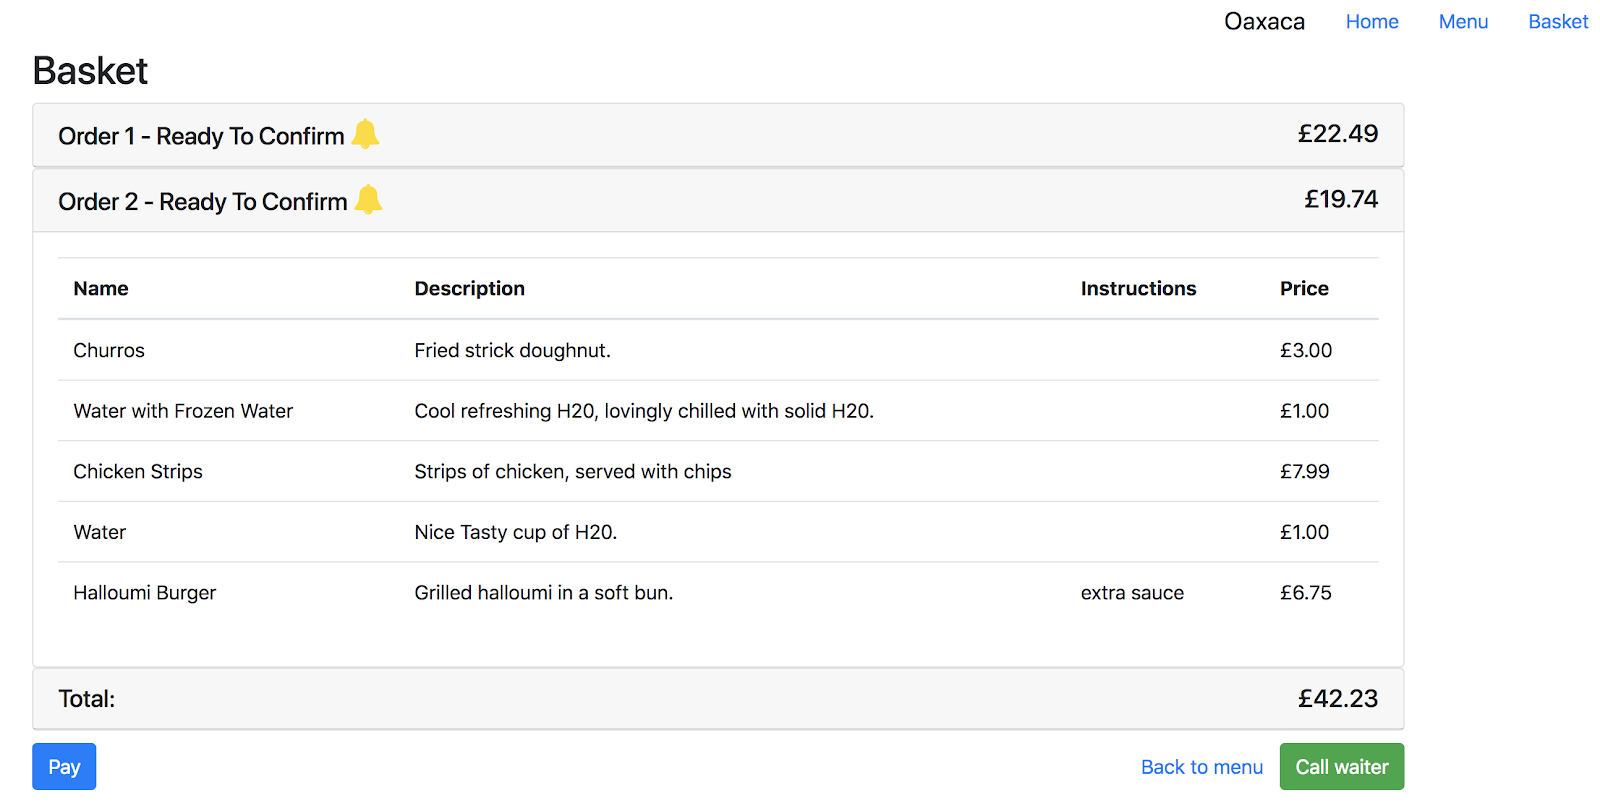
\includegraphics[width=15cm]{basket.png}
  \caption{The Customer's Basket Page}
  \label{fig:basket}
\end{figure}

\subsection*{Waiter}
\subsubsection*{Orders Page}

\subsubsection*{Edit Order View}

\subsection*{Kitchen}

\subsection*{Manager}
\subsubsection*{Manager Home Page}

\subsubsection*{Edit Menu Page}

\subsubsection*{Assign Tables Page}

\subsubsection*{Employee Page}

\section*{Server}

\section*{Database}

We have a database with 19 related tables, see Figure \ref{fig:data}. 

The database stores everything including the staff, the menu and the customers orders. 
It also stores the logged in sessions and the data needed for push notifications.
The database was designed to allow the user to start multiple orders and store them onto a transaction that allows the users to pay for all there orders in one go.

\begin{figure}[h]
  \centering
  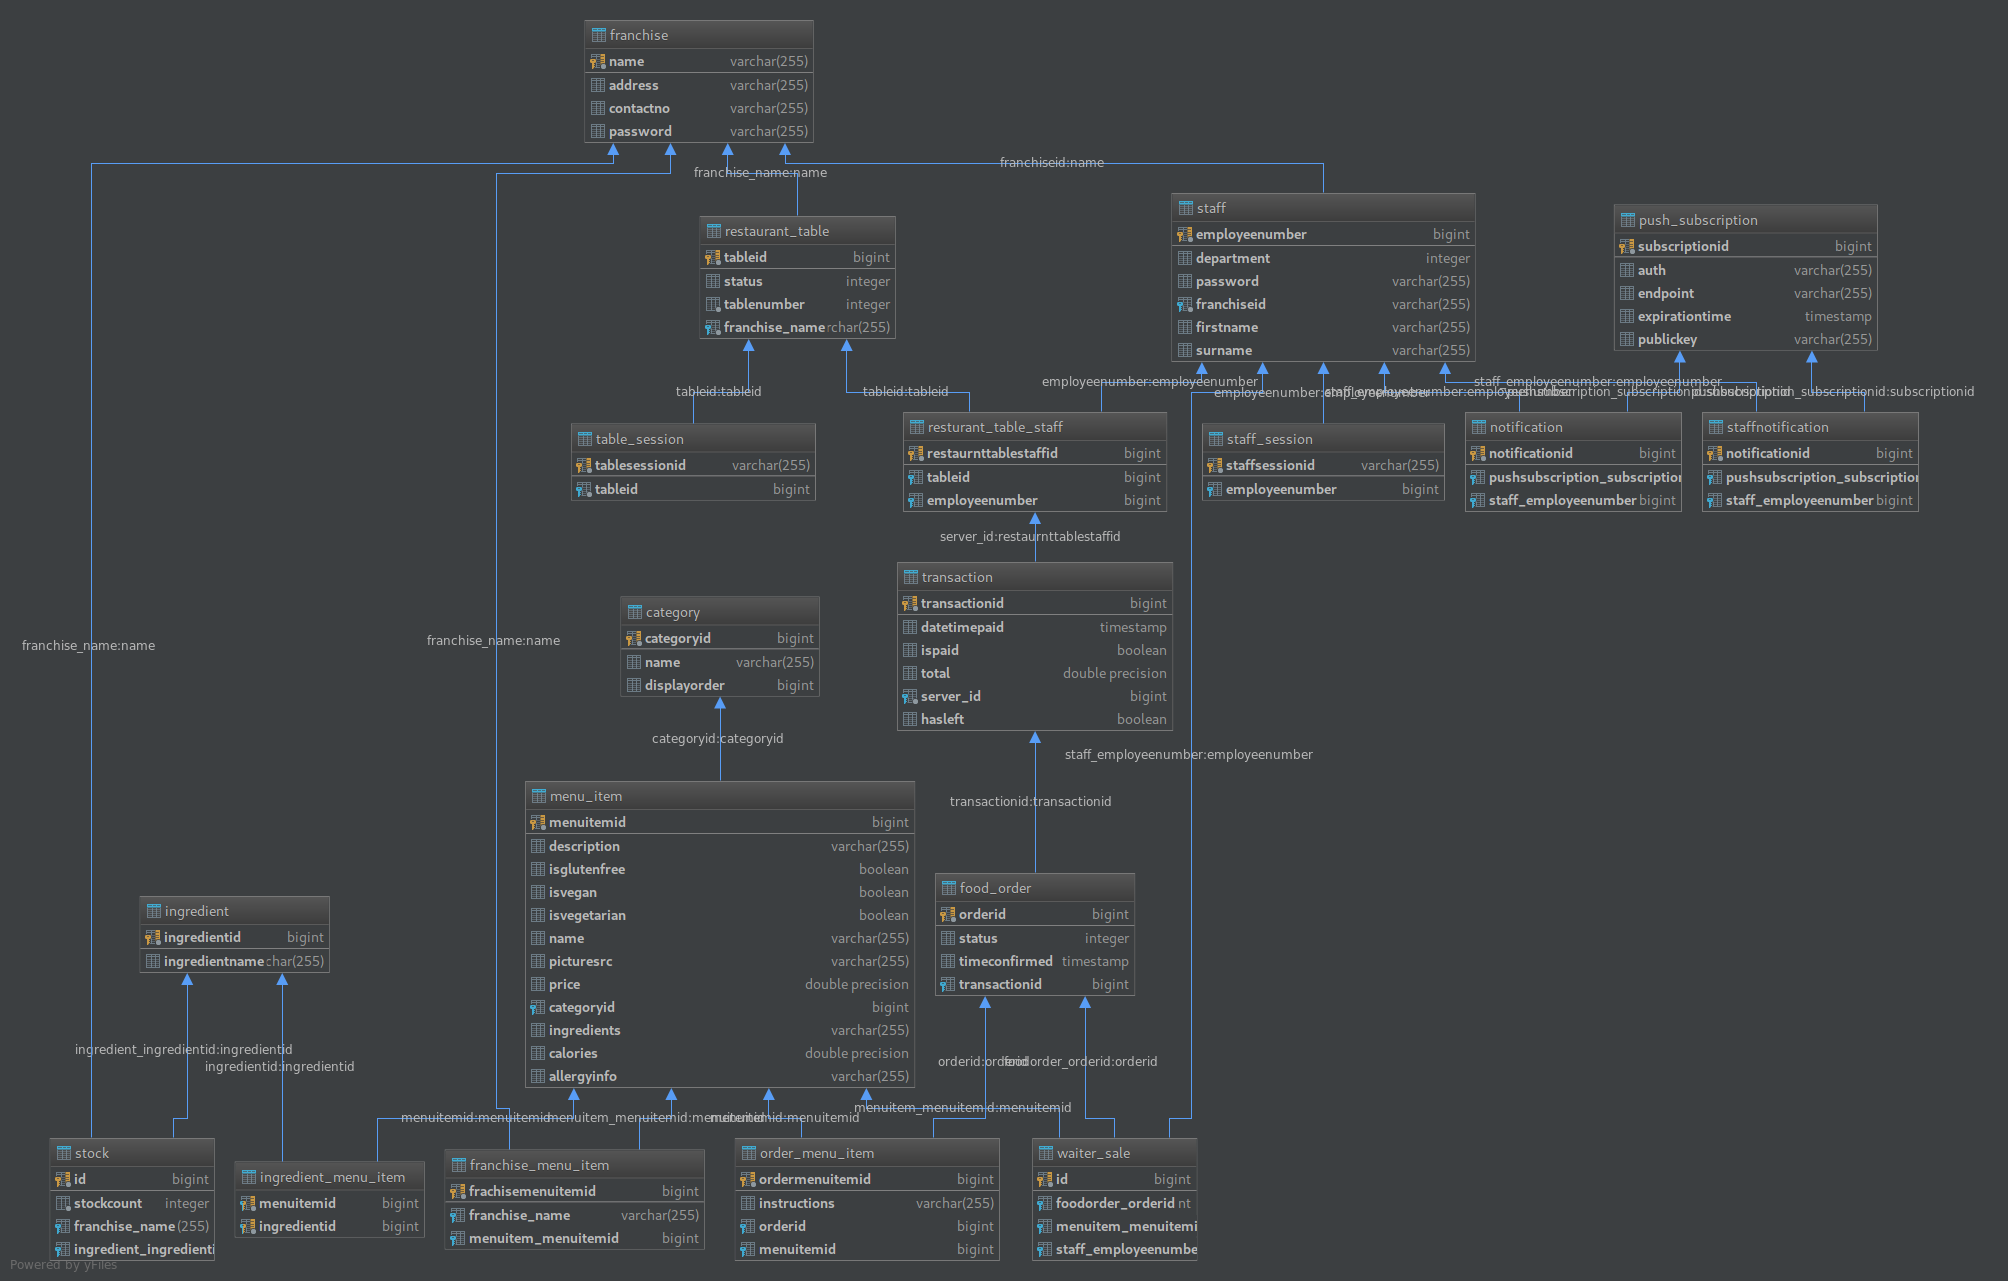
\includegraphics[width=15cm]{database.png}
  \caption{Generated by DataGrip}
  \label{fig:data}
\end{figure}

\chapter*{Description Of Packages}
\section*{PACKAGE}
\subsection*{Implemented Components}
\subsection*{Functionality}

\chapter*{User Stories}
\section*{Fully Completed}
These are the completed user stories.
\subsection*{Customer Stories}
\begin{itemize}
  \item Electronic Payment
  \item View Menu
  \item Ordering
  \item Menu Filtering
  \item Calling The Waiter
  \item Allergies And Calories
  \item Food Pictures
  \item Order Tracking
  \item Intuitive Ordering
\end{itemize}

\subsection*{Waiter Stories}
\begin{itemize}
  \item Notification For Delivery
  \item Cancel Order
  \item Order Times
  \item Payment Information
  \item Order Confirmation
  \item Table Assignment
  \item Mark Order as Delivered
  \item Client Needs Help
  \item Add Extra Sales
  \item Change Status Of An Order
\end{itemize}

\subsection*{Kitchen Stories}
\begin{itemize}
  \item Notify Waiters
  \item Confirmed Customer Order
  \item Order Times
\end{itemize}

\subsection*{Manager Stories}
\begin{itemize}
  \item Assign Tables
  \item Set Prices
\end{itemize}

\section*{Nearly Completed}
These stores are worthy of a mention as they are very nearly finished.

\subsection*{Manager Stories}
\begin{itemize}
  \item Adjust Menu:
    The only feature left uncompleted is uploading an image to the new menu item or when editing a menu item.
  \item Add Staff:
    The only feature left is the ability to reset a users password.
\end{itemize}

\chapter*{Statement of Relative Contribution}
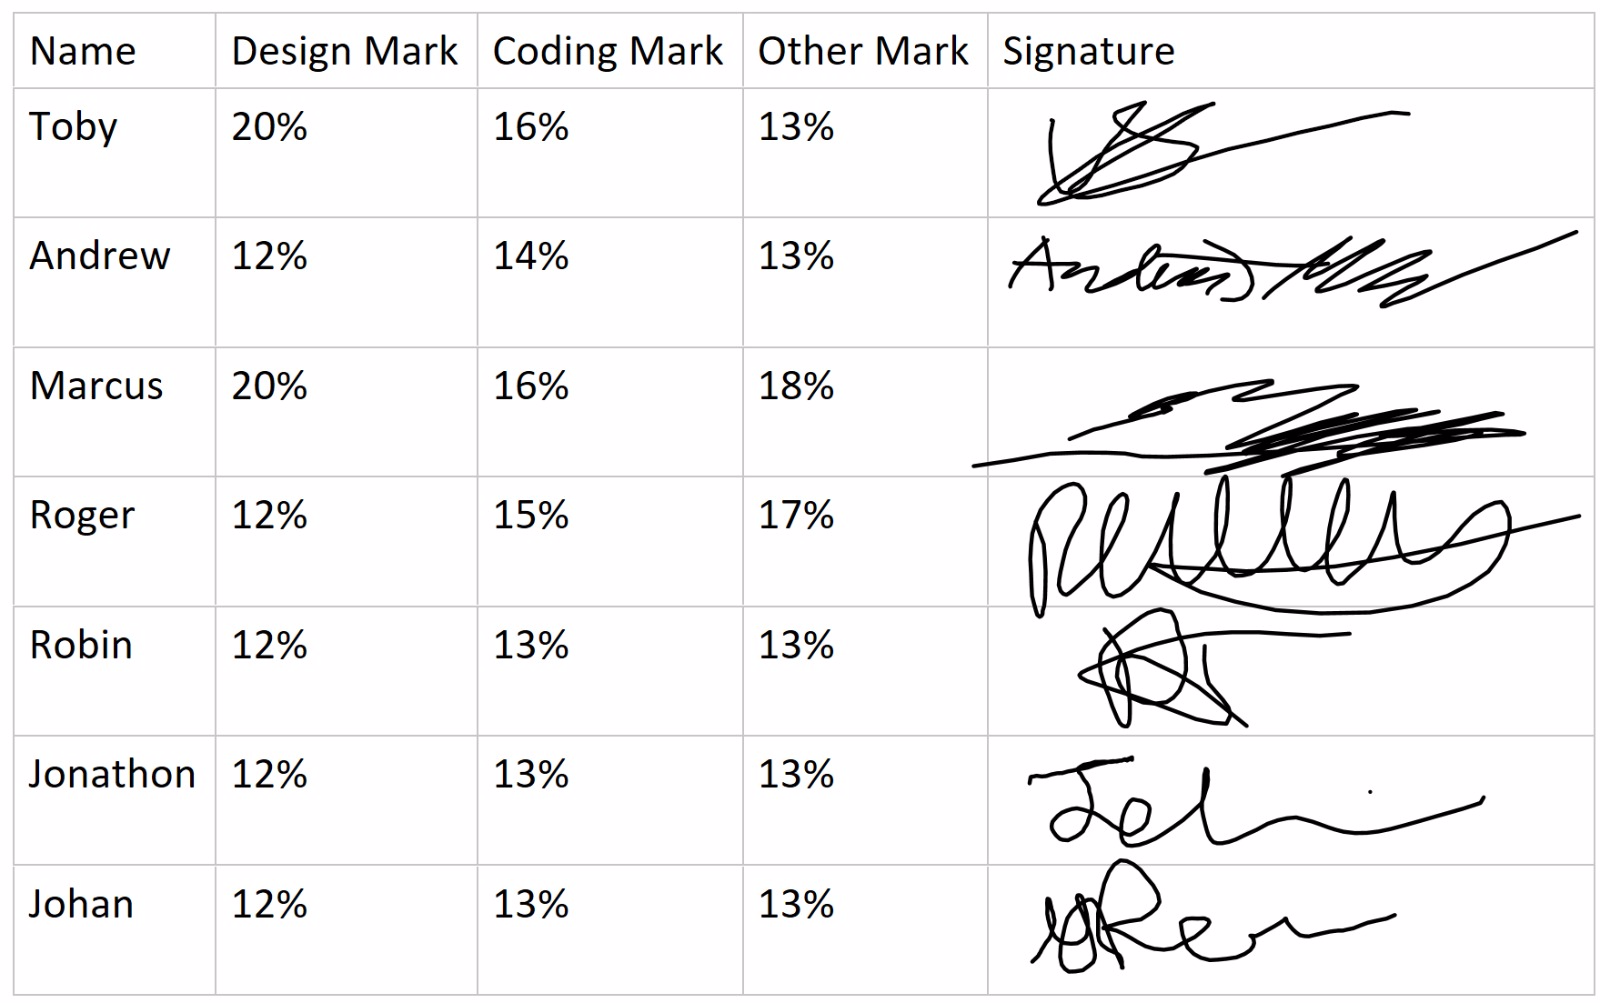
\includegraphics[width=15cm]{StateOfCont.png}

\end{document}
